\subsection{Energy Estimation}
\label{energy_model}


% The energy dispersion, also referred to as migration matrix, 
% can be seen in figure \ref{fig:energy}.
% It shows, that most predicted energies correlate well with the true event energies,
% but the model does not predict energies below 

% \begin{figure}
%     \centering
%     \captionsetup{width=0.6\textwidth}
%     \hspace*{0.15\textwidth}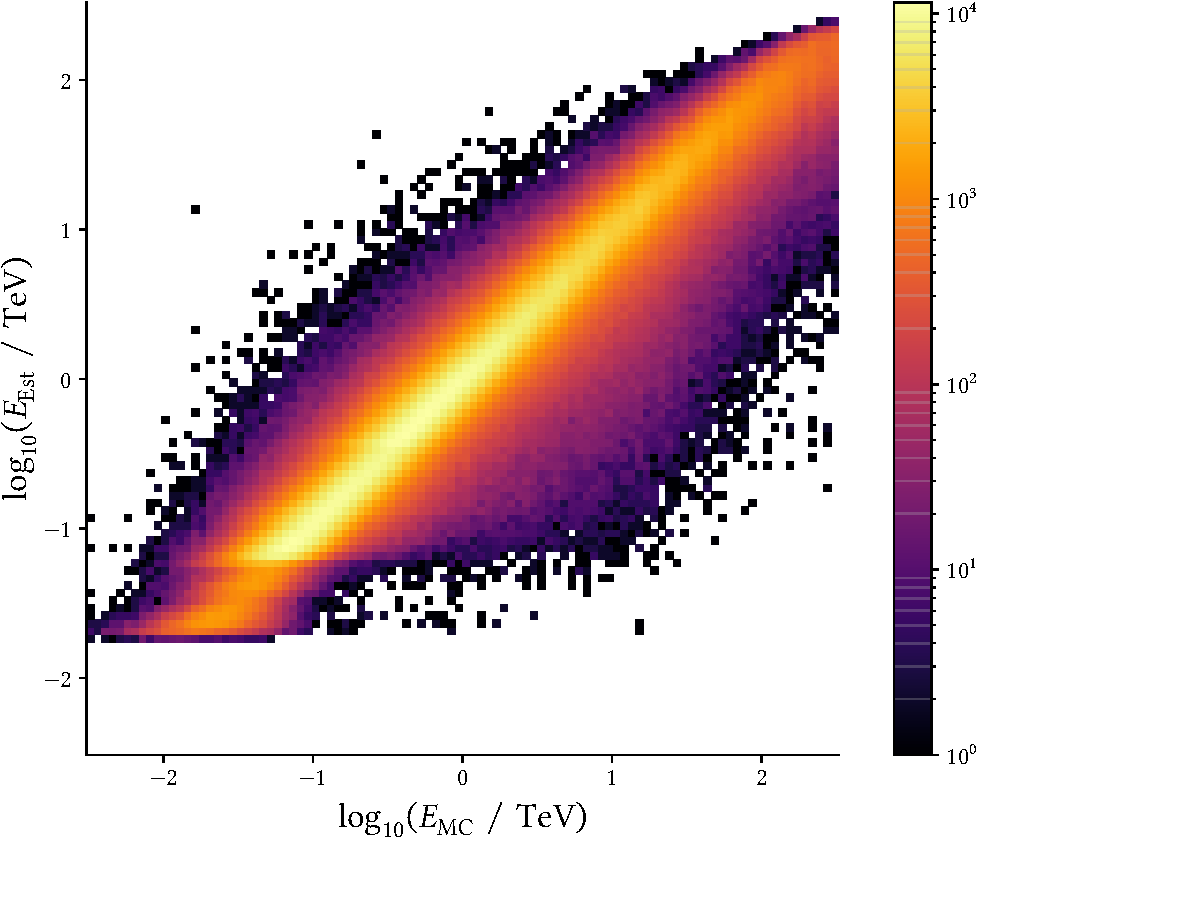
\includegraphics[page=1, width=.8\textwidth]{../analysis/plots/cross_val_reg_perf_plot.pdf}
%     \caption{Energy migration matrix with logarithmic color scale.}
%     \label{fig:energy}
% \end{figure}

Important information about the performance of a regressor model can be gained
looking at the estimation bias and resolution,
which are displayed in figure \ref{fig:energy_bias_res}.
Both describe the relative error of the prediction.
The bias is calculated as the median relative error and thus describes
whether the made predictions are on average matching the true values.
Resolution on the other hand is defined as
half the difference between the \num{15.9} and \num{84.1}th percentile
of the relative error distribution.
Other definitions for the resolution exist as well.
In both cases, values closer to 0 are better.
% $$Resolution = \frac{
%         Q_{84.1} (\Delta E_{rel})
%         - Q_{15.9} (\Delta E_{rel})
%     }
%     {2},$$
% with being the quantile of the distribution.

It can be noted, that the model tends to overestimate low and underestimate high energies.
This is not unexpected behaviour as events, that are recorded close to the threshold are increasingly
unregular. Low energy events need a certain brightness and high energy events suffer from
not being contained in the image.

\begin{figure}
    \centering
    \captionsetup{width=0.\textwidth}
    \includegraphics[page=3, width=.8\textwidth]{../analysis/plots/gamma_reg_perf_plot.pdf}
    \caption{Bias and resolution for the energy regressor model. 
    Lower absolute values are better. For small energies, 
    event energies get overestimated (positive bias), for high energies the estimations are too low (negative bias).
    The resolution improves with higher energies.}
    \label{fig:energy_bias_res}
\end{figure}

The feature importance is shown in figure \ref{fig:gh_features}.
Stereoscopic features and such, that describe the amount of
captured light, dominate, but the
spread in feature importance is very big for all features.
Features, that identify the telescope type also provide a lot of 
information, whereas timing features once again contribute very little.

\begin{figure}
    \centering
    \captionsetup{width=0.9\textwidth}
    \hspace*{-0.15\textwidth}\includegraphics[page=4, width=.8\textwidth]{../analysis/plots/gamma_reg_perf_plot.pdf}
    \caption{Feature importance for the energy regressor model. The light content of the image contains the most
    information about the event energy. The telescope identifying features and the
    stereoscopic features also add information.}
    \label{fig:gh_features}
\end{figure}
